\section{Maximum Matching im bipartiten Graphen}
Erklären Sie die Grundidee des Algorithmus zur Bestimmung eines Maximum Matchings in einem bipartiten Graphen.

\subsection*{Lösung}
Idee: Berechne eine Folge von Matchings $ M_0, M_1, ..., M_i $ mit 
\begin{enumerate}
    \item $ M_0 = \emptyset $
    \item $ M_{i+1} = M_i \oplus P_i $. $ P_i $ ist ein erweiternder Pfad für $ M_i $
    \item $ |P_i| \leq |P_{i + 1}| $. (Länge der erweiternden Pfade ist monoton wachsend)
    \item Alle verschiedenen $ P_i $ gleicher Länge sind knotendisjunkt. $ \Rightarrow $ Es existieren nur $ \sqrt{s} $ viele Paare solcher Pfade gleicher Länge.
\end{enumerate}

\paragraph{Initialisierung} Konstruiere $\hat{G}$ mit 2 neuen Knoten s und t richte die Kanten von A nach B. Der Abstand (Level) eines Knotens ist die Länge des Pfades von s aus. Hat ein Knoten v level[v]=-1, so ist er nicht mehr von s aus erreichbar.
\begin{figure}[h]
    \begin{center}
        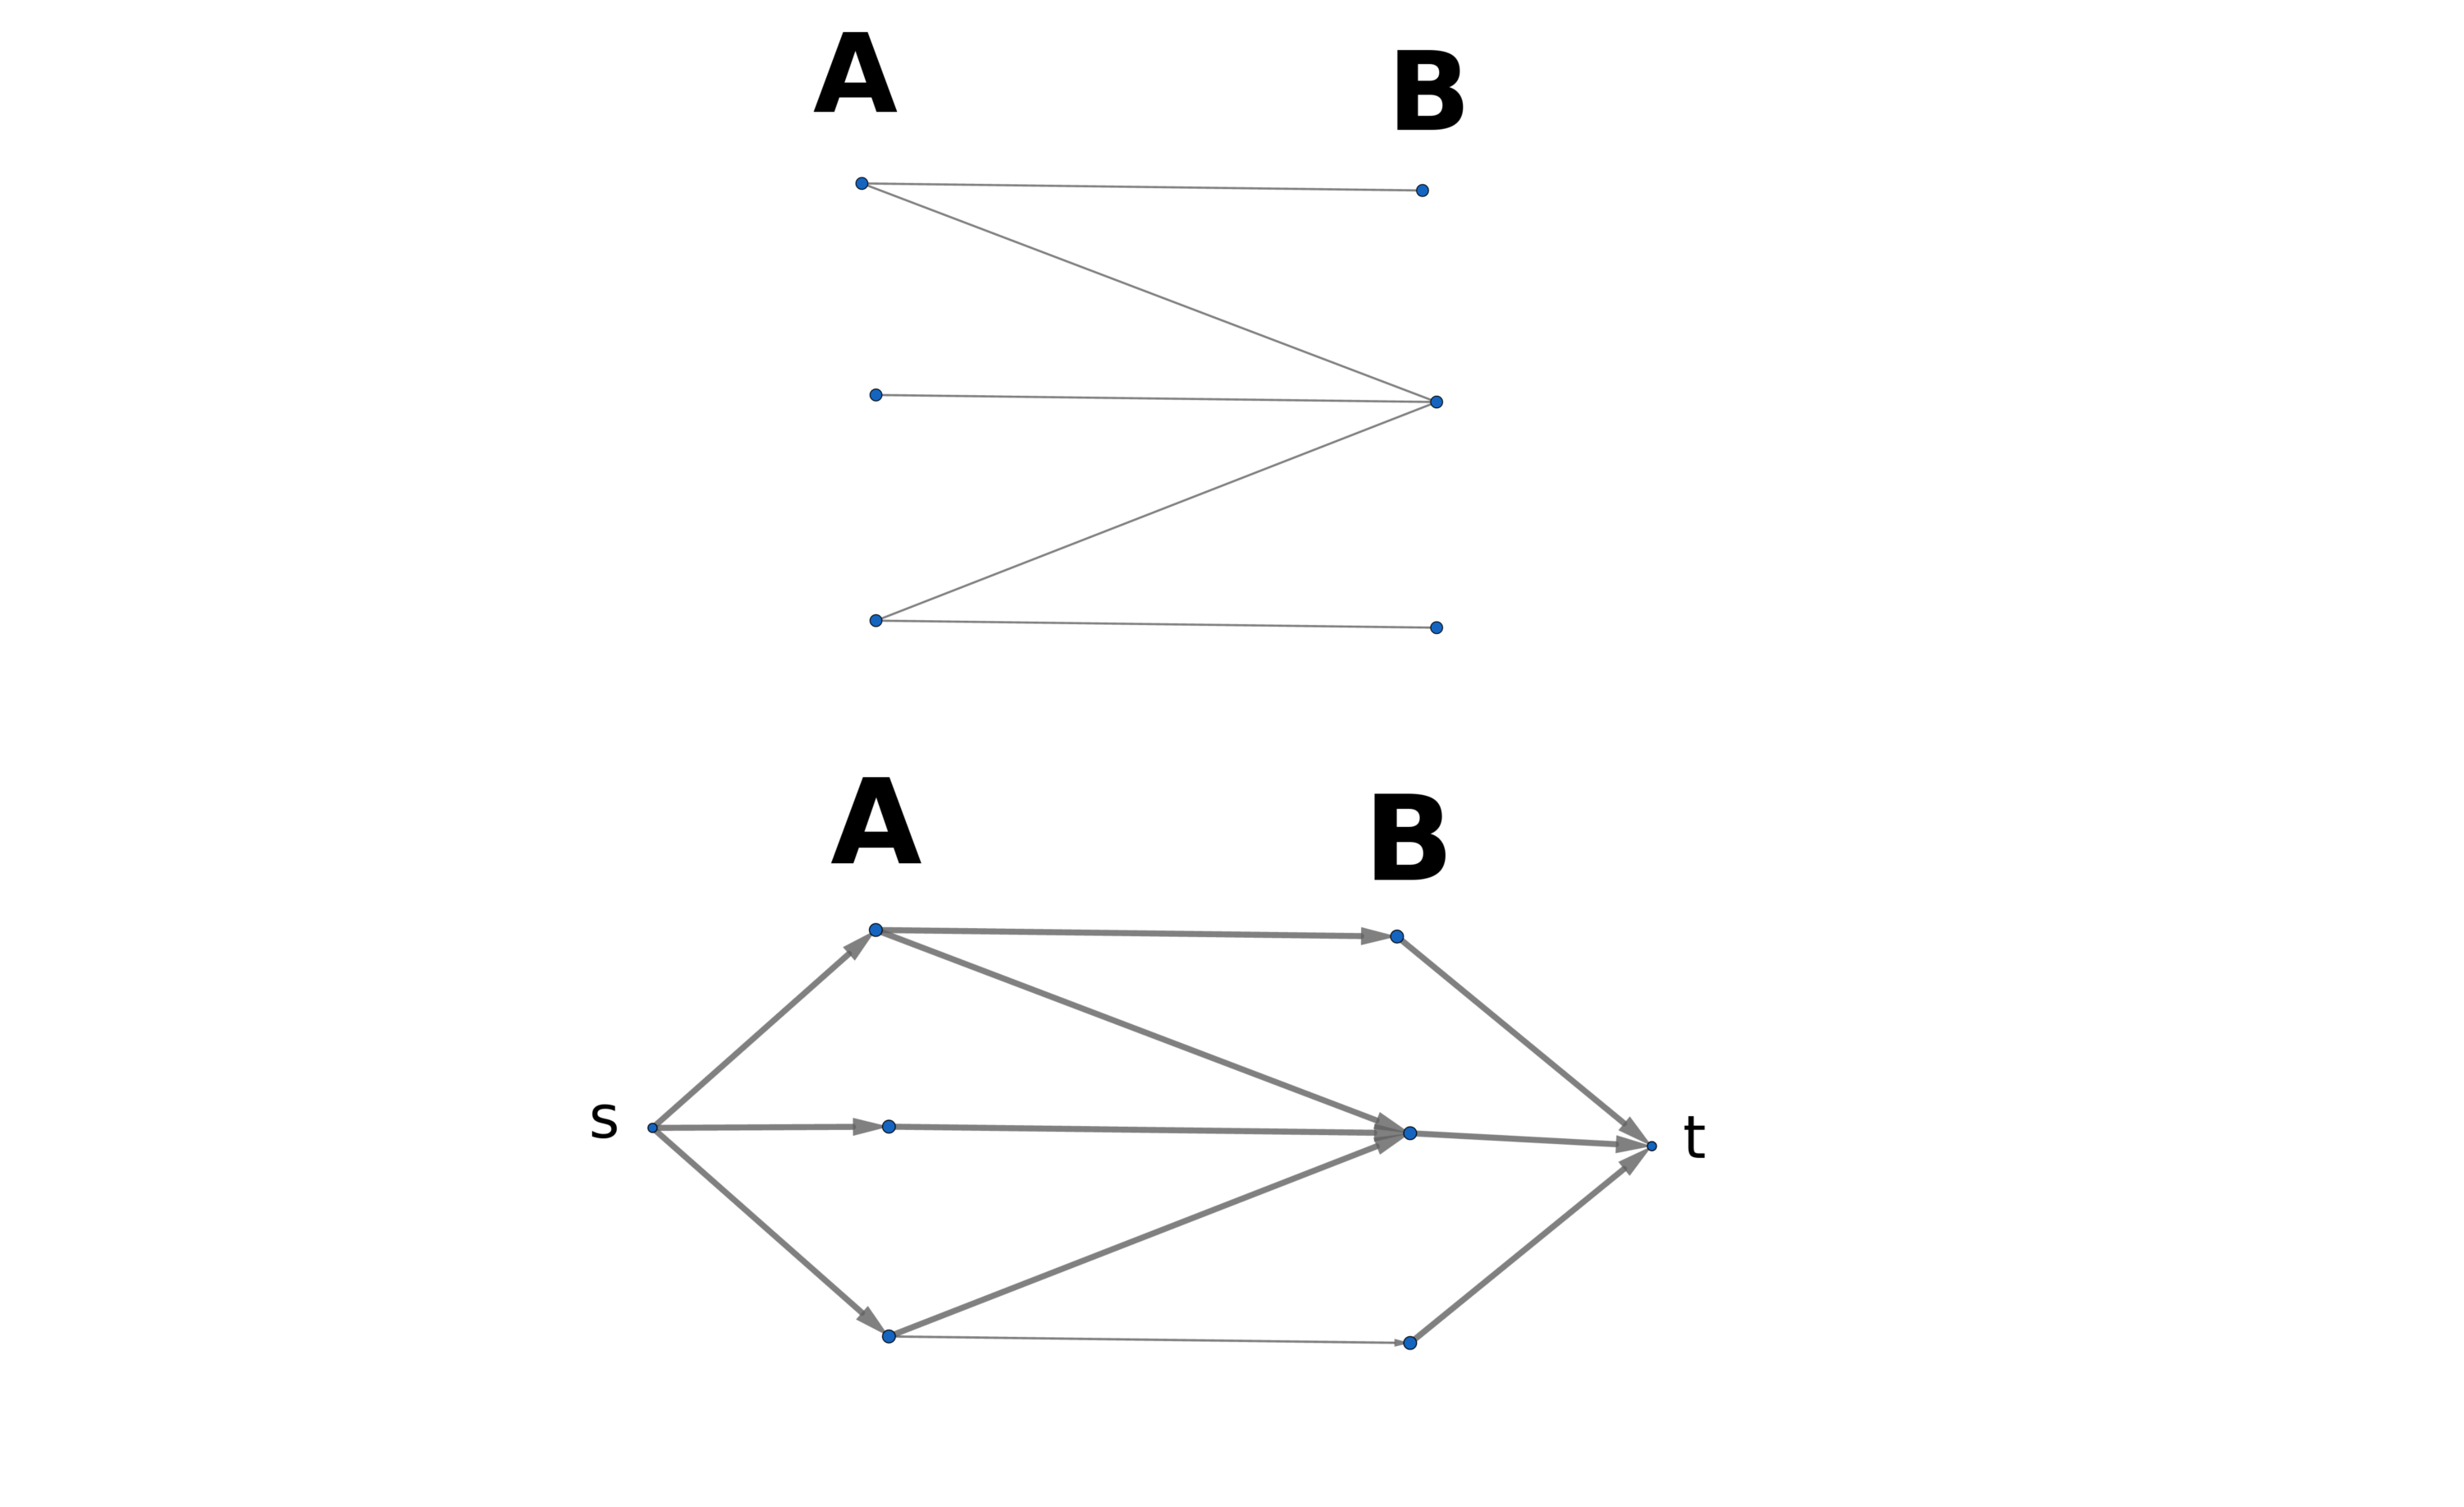
\includegraphics[width=10cm]{maxmatch}
        \caption{$ G \rightarrow \hat{G} $}
        \label{fig:}
    \end{center}
\end{figure}

\newpage
\paragraph{Innere Schleifen} Ausführung:
\begin{itemize}
    \item[] Solange ein Pfad von s anch t existiert, also level[t]$ \neq $-1
    \begin{itemize}
        \item[] Bestimme maximale Menge S von kürzesten knotendisjunkten erweiternden Pfaden (Phase), sodass für alle Kanten $ (v,w) $ von Pfaden in S gilt: level[v] = level[w]-1. Also jede Kante immer genau ein Level höher geht.
        \begin{itemize}
            \item Für jeden Pfad in S streiche die erste und letze Kante.
            \item Drehe alle anderen Kanten um.
        \end{itemize}
    \end{itemize}
\end{itemize}

\paragraph{Laufzeit}
$ O(\sqrt{n} m) $. da $ m > n $. $ \sqrt{n} $ Für die Anzahlt der Phasen und $ O(n+m) $ für Breiten und Tiefensuche zur Behandlung der Pfade.




